\documentclass{article}
\usepackage{amsmath}
\usepackage{amssymb}
\usepackage{amsfonts}
\usepackage{inputenc}
\usepackage{graphicx}
\title{Geometria e Algebra}
\begin{document}
\section{Geometria affine (richiami)}
\begin{flushleft}
	In geometria useremo dei spazi in cui lavoreremo che sono: retta, piano e spazio
\end{flushleft}
\begin{itemize}
	\item retta (euclidea) affine $(A^1)$
	\item piano affine ($\pi$ = piano) ($A^2$) $\pi \supseteq r$
	      \begin{flushleft}
		      $r_1$ e $r_2$ rette in $\pi$ sono:
	      \end{flushleft}
	      \begin{itemize}
		      \item inicidenti se $r_1 \cap r_2=\{ P \}$ (p punto)
		      \item parallele se $r_1 \cap r_2=\emptyset$ e se $ r_1 =r_2$
	      \end{itemize}
	\item spazio affine
	      \begin{flushleft}
		      I suoi sottoinsiemi notevoli sono:
	      \end{flushleft}
	      \begin{itemize}
		      \item punti (P)
		      \item rette (r)
		      \item piani ($\pi$)
	      \end{itemize}
	      \begin{flushleft}
		      Ora le varie regole
	      \end{flushleft}
	      \begin{itemize}
		      \item $\pi$ e $\pi$' nello spazio sono:
		            \begin{itemize}
			            \item incidenti se $\pi \cap \pi ' =r$
			            \item paralleli se $\pi \cap \pi ' =\emptyset$ e se $\pi = \pi '$
		            \end{itemize}
		      \item r e $\pi$ nello spazio sono:
		            \begin{itemize}
			            \item incidenti se $\pi \cap r = \{ P \}$
			            \item paralleli se $\pi \cap r = \emptyset$ e se $r \subseteq \pi$
		            \end{itemize}
		      \item r e r' sono:
		            \begin{itemize}
			            \item complanari se $\exists \pi: \quad \pi \subseteq r \land \pi \subseteq r'$
			            \item sgherbe se $r \cap r' = \emptyset$ e se $r \nparallel r'$
		            \end{itemize}
	      \end{itemize}
\end{itemize}

\section{Vettori orientati}
\begin{flushleft}
	I vettori orientati sono segmenti che partono da un punto di origine O e arrivano ad un punto P, se si vogliono avere piu' vettori
	questi devono partire tutti dallos stesso punto O
\end{flushleft}
\begin{flushleft}
	Def: Esiste una funzione $\Phi_o : A_o \rightarrow V_o^{1/2/3}$
\end{flushleft}
\begin{equation*}
	\Phi_o(P)=\overrightarrow{OP}
\end{equation*}
\begin{flushleft}
	Nota: La funzione $\Phi_o$ e' biettiva
\end{flushleft}
\subsection{Somma tra vettori}
\begin{flushleft}
	Def:$\forall v = \overrightarrow{OP}$ e $v' = \overrightarrow{OP}' in V_o^{1/2/3} \to \exists ! v''=\overrightarrow{OP}''$
\end{flushleft}
\begin{flushleft}
	Per la somma tra vettori si costruisce un parallelogramma con le parallele di entrambi i vettori di cui si intende sommare
	e poi si traccia una diagonale dal punto O fino al vertice che si formera e questa diagonale rappresentera' la somma di 2 vetttori
\end{flushleft}
\subsection{Proprieta' della somma in $V_o^{1/2/3}$}
\begin{enumerate}
	\item La somma e' associativa
	\item $\exists \overrightarrow{OO} \in V_o^{1/2/3}$ e' un elemento neutro della somma
	\item $\forall \overrightarrow{OP}, \exists \overrightarrow{OP}' \in V_o^{1/2/3}$ tale che
	      \begin{equation*}
		      \overrightarrow{OP} +\overrightarrow{OP}' = \overrightarrow{OO}=\overrightarrow{OP}' +\overrightarrow{OP}
	      \end{equation*}
	\item La somma e' commutativa
\end{enumerate}
\section{Moltiplicazione dello scalare}
\begin{flushleft}
	Def: $\forall v = \overrightarrow{OP} \in V_o^n$ (n=1,2,3)
	$\forall t \in \mathbb{R}, \exists !t: v=t*\overrightarrow{OP} \in V^n_o$ tale che
	$t*\overrightarrow{OP}=\overrightarrow{OP_t}$ dove $P_t \in A^t$ e' dato da
\end{flushleft}
\begin{itemize}
	\item Se $t=0$ $\to$ $P_t:= 0 \to t*\overrightarrow{OP}=\overrightarrow{OO}$
	\item Se $t>0$ $\to$ $P_t$ e' nella retta di $\overrightarrow{OP}$:
	      \begin{equation*}
		      \frac{lungh(\overrightarrow{OP_t})}{lungh(\overrightarrow{OP})} = t = |t|
	      \end{equation*}
	\item Se $t<0$:
	      \begin{equation*}
		      \frac{lungh(\overrightarrow{OP_t})}{lungh(\overrightarrow{OP})} = -t = |t|
	      \end{equation*}
\end{itemize}
\begin{flushleft}
	Tutto questo e' vero se $\overrightarrow{OP} \neq \overrightarrow{OO}$
	se invece $\overrightarrow{OP} = \overrightarrow{OO}$ allora $t*\overrightarrow{OO}=\overrightarrow{OO}$
\end{flushleft}
\begin{flushleft}
	Quindi esiste una funzione:
\end{flushleft}
\begin{itemize}
	\item $\mathbb{R}xV_o^n \to V_o^n$
	\item $(t,v) \to t*v$
\end{itemize}
\subsection{Proprieta' della moltiplicazione}
\begin{flushleft}
	$\forall v',v'' \in V_o^n$\\
	$\forall t',t'' \in \mathbb{R}$
\end{flushleft}
\begin{enumerate}
	\item $t' * (t''*v)=(t''*t')*v$
	\item $1*v=v$
	\item $t' + (t''+v)=(t''+t')+v$
	\item $t*(v'+v'')=(t*v')+(t*v'')$
\end{enumerate}
\section{Riferimenti affini e coordinate}
\subsection*{[n=1]}
\begin{flushleft}
	Fisso $O \in A^n$ e fisso $\overrightarrow{i} \in V^n_O$, con $\overrightarrow{i} \neq \overrightarrow{OO}$
\end{flushleft}
\begin{flushleft}
	Allora $ \forall v = \overrightarrow{OP} \in V^1_O,\exists ! x\in \mathbb{R}:v= \overrightarrow{OP} = x* \overrightarrow{i}$
\end{flushleft}
Quindi
\begin{equation*}
	|x|=\frac{lungh(\overrightarrow{OP})}{lungh(\overrightarrow{i})}
\end{equation*}
\begin{flushleft}
	Tale x si dice coordinata di $\overrightarrow{OP}$ (o del punto P) e il vettore di riferimento affine e' $(o;\overrightarrow{i})$
\end{flushleft}
\begin{flushleft}
	il segno di x dipende da dove si trova il vettore OP rispetto ad il vettore i
\end{flushleft}
\begin{itemize}
	\item + se si trova nella stessa parte del vettore di OP
	\item - se si trova nella parte opposta del vettore di OP
\end{itemize}
\subsection*{[n=2]}
\begin{flushleft}
	Fisso $O \in A^2$ e fisso $\overrightarrow{i},\overrightarrow{j} \in V^2_O$, con $\overrightarrow{i},\overrightarrow{j}$ non multipli tra di loro
\end{flushleft}
\begin{equation*}
	V_O^2 \iff \mathbb{R}^2
\end{equation*}
\begin{equation*}
	(x,\overrightarrow{i})+(y,\overrightarrow{j}) \leftarrow (x,y)
\end{equation*}
\begin{flushleft}
	Allora $\forall \overrightarrow{v}=\overrightarrow{OP} \in V^2_O \quad \exists ! (x,y) \in \mathbb{R}^2$ tale che
\end{flushleft}
\begin{equation*}
	\overrightarrow{v}=\overrightarrow{OP}=(x,\overrightarrow{i})+(y,\overrightarrow{j})
\end{equation*}
\subsection*{[n=3]}
\begin{flushleft}
	Fisso $O \in A^3$ e fisso $\overrightarrow{i},\overrightarrow{j},\overrightarrow{k} \in V^3_O$
\end{flushleft}
\begin{equation*}
	V_O^3 \iff \mathbb{R}^3
\end{equation*}
\begin{equation*}
	x*\overrightarrow{i}+y*\overrightarrow{j}+z*\overrightarrow{k} \leftarrow (x,y,z)
\end{equation*}
\begin{flushleft}
	$\overrightarrow{i},\overrightarrow{j},\overrightarrow{k}$ non devono essere complanari
\end{flushleft}
\begin{flushleft}
	Def: (x,y,z) sono coordinate di $v=\overrightarrow{OP}$ (o di P)
\end{flushleft}
quindi possiamo dedurre questo
\begin{equation*}
	\mathbb{R}^n \iff V_O^n
\end{equation*}
\section{Equazioni vettoriali di rette e piani}
\begin{flushleft}
	L'equazione vettoriale di una retta r,
	$(O,\overrightarrow{i},\overrightarrow{j},\overrightarrow{k})$ e' riferimento affine (in $A^2,A^3$)
\end{flushleft}
\begin{flushleft}
	$\exists ! r_0 : r_0 || r, O \in r_0$
\end{flushleft}
\begin{flushleft}
	$ Q \in r_0, Q \neq O, \overrightarrow{v_2}=\overrightarrow{OQ} \quad (\neq \overrightarrow{OO})$
\end{flushleft}
\begin{flushleft}
	$\forall P \in A^{2/3}$ si ha $ P \in r$ e $P_0 \neq P \iff \overline{P_0 P} || r_0 \quad \exists ! P' \in r_0$
\end{flushleft}
\begin{flushleft}
	$\to \overrightarrow{OP} = \overrightarrow{OP_0} + \overrightarrow{OP'} (\in V_0^{2/3})$
\end{flushleft}
\begin{itemize}
	\item $\overrightarrow{OP}$ = il valore e' variabile
	\item $\overrightarrow{OP_0}$ = il valore e' fisso
	\item $\overrightarrow{OP'}$ = il valore e' variabile
\end{itemize}
\begin{flushleft}
	$\overrightarrow{OP'}$ e' sulla retta $r_0$ che ha riferimento affine $(O;\overrightarrow{v_r})$
\end{flushleft}
\subsection*{Equazione vettoriale di una retta}
\begin{equation*}
	r = \{ P \in A^{2/3} | \exists t \in \mathbb{R}: \overrightarrow{OP}=\overrightarrow{OP_0}+t*\overrightarrow{v_r} \}
\end{equation*}
\begin{flushleft}
	Def:  $\overrightarrow{v_r}$ si dice vettore direttore
\end{flushleft}
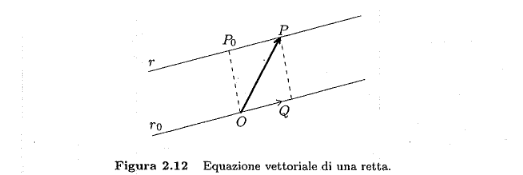
\includegraphics[bb=0 0 350 100]{equazione-retta-v.png}
\subsection*{Equazione vettoriale per piani}
\begin{flushleft}
	$\forall \overrightarrow{v} \in V^3_0, \exists ! (s,t,d):
		s\overrightarrow{i} + t\overrightarrow{j} + d\overrightarrow{k} = \overrightarrow{r}$
\end{flushleft}
\begin{flushleft}
	questi vettori non devono essere complanari
\end{flushleft}
\begin{flushleft}
	$ \exists \pi_0 :\pi_0 || \pi \land O \in  \pi_0$
\end{flushleft}
\begin{equation*}
	P\in \pi \iff \overrightarrow{OP'} \subseteq \pi_0 \iff \overrightarrow{OP'}=\overrightarrow{OP} - \overrightarrow{OP_0} \quad \in V^2_0
\end{equation*}
\subsubsection*{Equazione vettoriale di $\pi$}
\begin{equation*}
	\exists ! (s,t) \in \mathbb{R}^2:\overrightarrow{OP}=\overrightarrow{OP_0}+s\overrightarrow{v}+t\overrightarrow{w}
\end{equation*}

\section{Campi}
\begin{flushleft}
	Def: Campi sono insiemi di numeri in cui si fanno operazioni
\end{flushleft}
\begin{flushleft}
	K e' un campo se e' un insieme con 2 operazioni
\end{flushleft}
\begin{itemize}
	\item + : $KxK \to K$
	\item * : $KxK \to K$
\end{itemize}
\subsection{Somma nei campi}
\begin{enumerate}
	\item La somma e' assiciativa
	\item $\exists O_k \in \mathbb{K} : x+O_k=x \quad \forall x\in \mathbb{K}$
	\item $\forall x \in  \mathbb{K},\exists (-x) \in \mathbb{K}:x+(-x)=O_k$
	\item x+y=y+x $\forall x,y \in \mathbb{K}$
\end{enumerate}
\subsection{Prodotto nei campi}
\begin{enumerate}
	\item Il prodotto e' assiciativa
	\item $\exists 1_k \in \mathbb{K} : x*1_k=x \quad \forall x\in \mathbb{K}$
	\item $\forall x \in  \mathbb{K},\exists x^{-1} \in \mathbb{K}:x*x^{-1}=1_k$
	\item x+y=y+x $\forall x,y \in \mathbb{K}$
\end{enumerate}
\begin{itemize}
	\item D $\rightarrow$ x*(y+z)=(x*y)+(x*z)
	\item D $\leftarrow$ (x+y)*z)=(z*y)+(x*z)
\end{itemize}
\subsection*{Esempi}
\begin{enumerate}
	\item $\mathbb{N}:$ no , $\mathbb{Z}: $ no
	\item $\mathbb{Q}:$ si, $\mathbb{R}: $ si
	\item $\mathbb{Z}_n$ e' un campo se e soltanto se se n e' un numero primo
\end{enumerate}
\section{Spazi Vettoriali}
\begin{flushleft}
	Def: spazio veottoriale su K e' un insieme V con 2 funzioni:
\end{flushleft}
\begin{itemize}
	\item +: $VxV \to V \quad \quad (v',v'') \to v' + v''$
	\item *: $KxV \to V \quad \quad (k,v)\to kv$
\end{itemize}
\subsection*{Proprieta'}
\subsubsection*{Somma}
\begin{enumerate}
	\item Associativa $\forall v,w,u \in \mathbb{V}$
	\item $\exists O_v \in V: $ elemento neutro $\forall v \in \mathbb{V}$
	\item $\forall v \in  \mathbb{V},\exists (-v) \in \mathbb{V}:v+(-v)=O_v$
	\item v+w=w+v $\quad \forall v,w \in \mathbb{V}$
\end{enumerate}
\subsubsection*{Prodotto}
\begin{enumerate}
	\item Associativa $\forall v,w,u \in \mathbb{V}$
	\item $\exists 1_v \in V: $ elemento neutro $\forall v \in \mathbb{V}$
	\item $\forall v \in  \mathbb{V},\exists v^{-1} \in \mathbb{V}:v+v^{-1}=O_v$
	\item v*w=w*v $\quad \forall v,w \in \mathbb{V}$
\end{enumerate}
\begin{itemize}
	\item $k*(v_1+v_2)=(k*v_1)+(k*v_2) \quad \quad \forall v_1,v_2 \in \mathbb{V}, \forall k \in \mathbb{K}$
	\item $v*(k_1+k_2)=(v*k_1)+(v*k_2) \quad \quad \forall k_1,k_2 \in \mathbb{K}, \forall v \in \mathbb{V}$
\end{itemize}
\begin{flushleft}
	Def: $\forall$ spazio vettoriale V (su K) e' un sotto spazio di V e' un sottoinsieme
\end{flushleft}
\begin{flushleft}
	Un $W \subseteq V$ e' sottospazio (vettoriale) se:
\end{flushleft}
\begin{equation*}
	W+W \subseteq W \quad K*W \subseteq W \quad W \neq \emptyset
\end{equation*}
\begin{flushleft}
	($W\leq V$) e' un rafforzamento di $\subseteq$
\end{flushleft}
\subsubsection*{Lemma:}
\begin{flushleft}
	Se V e' un sottospazio vettoriale e $W \leq V$ allora $W$ e' uno spazio vettoriale con somma e prodotto dati da quelli di V ristretti ai vettori di $W$
\end{flushleft}
\textbf{Esempi:}
\begin{enumerate}
	\item $Der(a,b)=\{ f \in \mathbb{R}^{(a,b)} | \text{ f e' derivabile } \}$
	\item $C^0(a,b)= \{ f \in \mathbb{R}^{(a,b)} | \text{ f e' continua } \}$
	      \begin{equation*}
		      Der(a.b) \subseteq C^0(a,b) \land Der(a,b) \leq C^0(a,b)
	      \end{equation*}
	\item $Conv(\mathbb{R}^{\mathbb{N}}) = \{ \{a\}_n | \exists \text{ limite $\in \mathbb{R}$ (convergente)}\}$
	      \begin{flushleft}
		      e' sottospazio vettoriale di $\mathbb{R}^{\mathbb{N}}$ perche' se sommiamo 2 successioni il limite della somma sara' lo stesso.
		      Se moltiplichiamo uno scalare per una successione il limite e' ancora lo stesso
	      \end{flushleft}
	\item $Inf(\mathbb{R}^{\mathbb{N}}) =\{ \{ a \}_n \in \mathbb{R}^{\mathbb{N}} | \exists \text{ lim $a_n$ = 0 } \}$
	      \begin{flushleft}
		      e' sottospazio vettoriale di $Conv(\mathbb{R}^{\mathbb{N}})$
	      \end{flushleft}
\end{enumerate}
\begin{flushleft}
	Def: $\forall$ spazio vettoriale , $\forall v,...,v_n \in V$ sia
\end{flushleft}
\begin{equation*}
	\sigma_{v_1,...,v_n}: K^n \to V \quad \text{ data da}
\end{equation*}
\begin{equation*}
	\sigma_{v_1,...,v_n} (K_1,...,K_n) = \sum^n_{i=1} k_i v_i \quad (\in V)
\end{equation*}
\begin{flushleft}
	questo si dice combinazione lineare di $v_1,...,v_n$ con coefficenti $K_1,...,K_n$
\end{flushleft}
\begin{equation*}
	\text{span}(v_1,...,v_n)=\text{Immagine}(\sigma_{v_1,...,v_n}) = \text{sottospazio generato da }(v_1,...,v_n)
\end{equation*}
\textbf{Lemma}
\begin{flushleft}
	Span($v_1,...,v_n$) e' un sottospazio vettoriale di V
\end{flushleft}



\end{document}

